\subsection{Python als Progrmmiersprache}

Nach dem Scheitern seiner ersten Programmiersprache, entwickelte Guido van Rossum die Sprache Python, dabei wollte er alle Fehler, die er beim Entwickeln von ABC gefunden hat, verbessern. Daher basieren auch die Stukturen und Konventionen von Python auf Unix, ohne an Unix gebunden zu sein. 

Python unterscheidet sich in vielen Punkten zu anderen Sprachen, unteranderem dass sie viel Wert auf Lesbarkeit gibt. Die auffälliste davon ist, dass Einrückungen Codeblöcke unterteilt anstatt eine Art von Klammern. Dafür gibt es zwei Gründe:

\begin{itemize}
    \item Es macht den Code kürzer und er wirkt nicht unnötig ausgeschmückt, daher braucht man eine kürzere Aufmerksamkeitsspanne um den Sinn einer Codestelle nachvollziehen zu können.
    \item Die Stuktur des Codes ist vereinhaltlicht, was es einfacher macht Projekte von anderen zu verstehen.
\end{itemize}

Außerdem werden dem Entwickler in vielen Entscheidungen leichter gemacht, da unnötige Möglichkeiten entfernt wurden, das heißt, dass es meisten nur eine offensichtliche Art und Weise gibt, etwas zu implementieren. Dazu kommt noch die Nutzung von Spezialzeichen, es werden nur Zeichen unterstützt, die den meisten bereits bekannt sind und dessen Operation Sinn machen. \cite{PythonGVR:online}

Dies beantwortet jedoch nicht die Frage ''Wieso ist Python die beliebteste Sprache für \gls{ml}?''. Die Antwort darauf ist, dass die Sprache nicht nur triviale Aufgaben bereits vorimplementiert, sonder auch, dass die meisten ML Funktionen in Python Libraries zusammengefasst sind. Daher muss man als Neuanfänger oder Fortgeschrittener keine bereits gelösten Probleme von Grund auf noch einmal angehen.

\subsection{Notebooks}

Da es bei \gls{ml} es öfters dazu kommt, dass bestimmte Codeblöcke oft wiederholt ausgeführt werden, kann man mit Hilfe von Notebooks diese einzelen ausführen. Zum Beispiel beim Analysieren eines Datensatzes oder schnell kleine Änderung am geplanten Vorgehen vorzunehemen.

Diese Codeblöcke können entweder Code, Texte oder Grafiken beinhalten, diese werden fortlaufend mit einer Nummer versehen und die Ausgabe/Grafik erscheint direkt unter dem Code.

\begin{figure}[H]
    \centering
    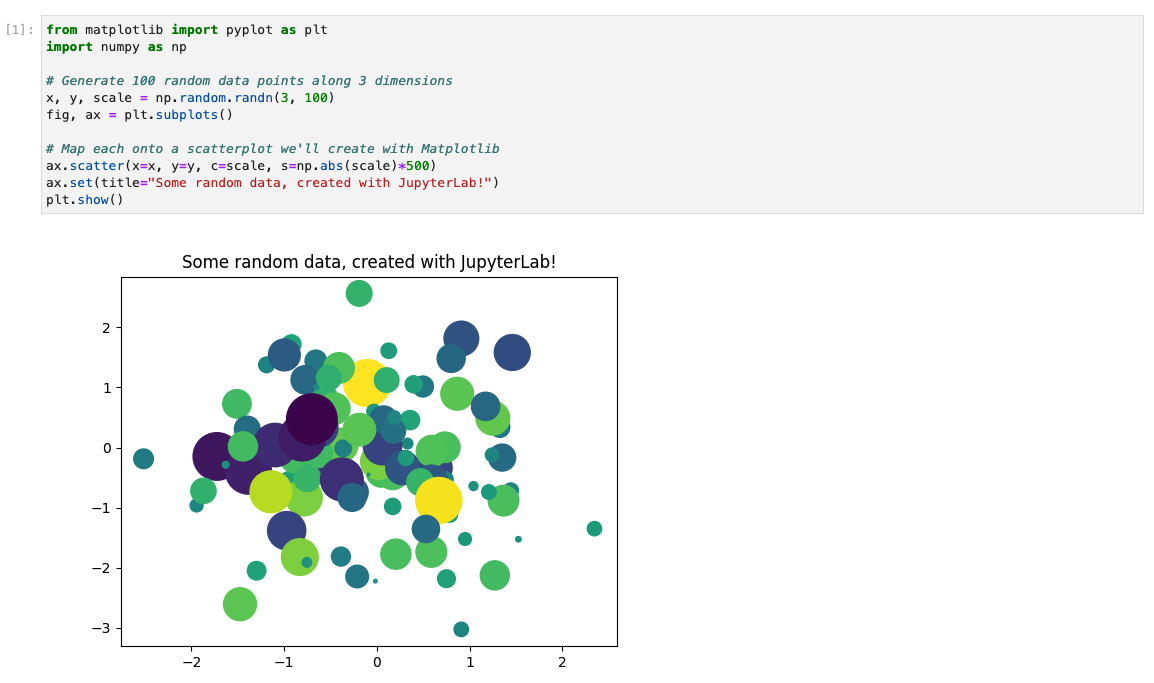
\includegraphics[scale=0.4]{sections/machine-learning/images/jupyter-notebook.png}
    \caption{Beispiel für ein Notebook mit Code und Ausgabe mit Jupyter Notebook}
\end{figure}

Diese Notebooks kann man entweder lokal starten oder auf diversen Webseiten online benutzten, dann wird auch der Code auf den Servern dieser Notebookseiten ausgeführt. Dies kann von großem Vorteil sein, da oft generierte Grafiken sehr viel Leistung in Spruch nehmen. Außerdem werden die Ergebnisse/Ausgaben gespeichter und man muss nicht bei jedem Neuladen jeden Codeblock neu ausführen. 

\subsection{Libraries}

\paragraph{Pandas}

Bevor der eigentliche ML-Prozess beginnen kann, müssen die Daten als Erstes analysiert werden und dafür ist die Library ''pandas'' geeignet . Neben der Analyse ist pandas auch in der Datenmanipulation sehr hilfreich, da die vordefinierten Funktionen nicht nur leicht und verständlich sind, sondern auch für echte Daten aus der Welt gedacht.

Zu den zwei Hauptdatentypen von pandas gehörten Dataframes und Series.

\subparagraph*{Series} sind eindimensionale Arrays, welche aus verschiedenen Datentypen bestehen können. Mithilfe von einer ID kann man auf jeden Eintrag in der Series zugreifen, diese sind entweder mitgegeben worden oder von pandas generiert (aufsteigende Zahl beginnend bei 0).

Mit der Methode \lstinline!pandas.Series(data)! kann man diese Datentypen in Series umwandeln: 

\begin{itemize}
    \item Dictionary
    \item ndarray
    \item Skalarwert
\end{itemize}

\subparagraph{Dataframes} sind zweidimensionale Tabllen mit verschiedenen Datentypen als Spalten. Sie sind vergleichbar mit Datenbanktabellen oder mit einem Dictionary mit dem Datentyp Series als Value. 
    
Jede Zeile beinhaltet eine ID, falls diese nicht vergeben ist, wird von pandas eine generiert und mittels dieser ID kann man dann auf bestimmte Zeilen zugreifen. Das gleiche Prinzip gilt bei den Spalten, wo man mit der Spaltenbezeichnung auf jeden Wert der Zeilen assoziiert mit dieser Spalte zugreifen kann. 

pandas bietet beim Erstellen von Dataframes mehrere Möglichkeiten an:

\begin{itemize}
    \item Einlesen einer Datei (*.json, *.html, *.sql, *.xlsx, ...)
    
    Am Beispiel einer .csv-Datei: \lstinline!pandas.read_csv(FILENAME)!
    \item Dictionaries
    
    \lstinline!pandas.DataFrame.from_dict(DICT_VARIABLE)!
    \item Series
    
    \lstinline!pandas.Series.to_frame(SERIES_VARIABLE)!
    \item Anderes Dataframe
\end{itemize}

Das Benutzen von pandas ersparrt sehr viel Zeit und ermöglicht den schnellsten Weg zu einem Ergebniss mit diesen Funkionalitäten:

\begin{itemize}
    \item Löschen und Ersetzen von fehlenden Daten, welches in %Preprocessing erklären 
    \item HInzufügen und Löschen von Spalten in Dataframes
    \item Gruppierung von Daten
    \item Koventierung in NumPy oder andere Python Objekte
    \item ...
\end{itemize}

\paragraph{Seaborn} ist eine auf Matplotlib basierende Visualisierungslibrary.

Auch wenn das Analysieren der Daten eine grobe Einschätzung ermöglicht, ist es für das menschliche Auge besser diese Daten in Grafiken und Diagrammen visualisiert zu sehen. Auch bei größeren Datensätzen wird mit der Visualisierung ermöglicht, dass Zusammenhänge, Muster oder Ausreißer besser erkannt werden.

Bei der Auswertung ist es wichtig die Datenverbreitung zu beachten, da die Auswahl von Daten ein Diagramm stark beeinflussen kann.

Da jede Art von Diagrammen Vor- und Nachteile hat, ist es wichtig die Daten in verschiedenen Diagrammtypen darzustellen. Eine Auswahl von möglichen Plots ist hier aufgelistet:

\begin{itemize}
    \item Scatter Plot
    \item Box Plot, ermöglicht das Ablesen von Ausreißern
    \item Violin Plot
    \item Swarm Plot
    \item Histogram
    \item Bar Plot
    \item Dist Plots
\end{itemize}

\begin{figure}[H]
    \centering
    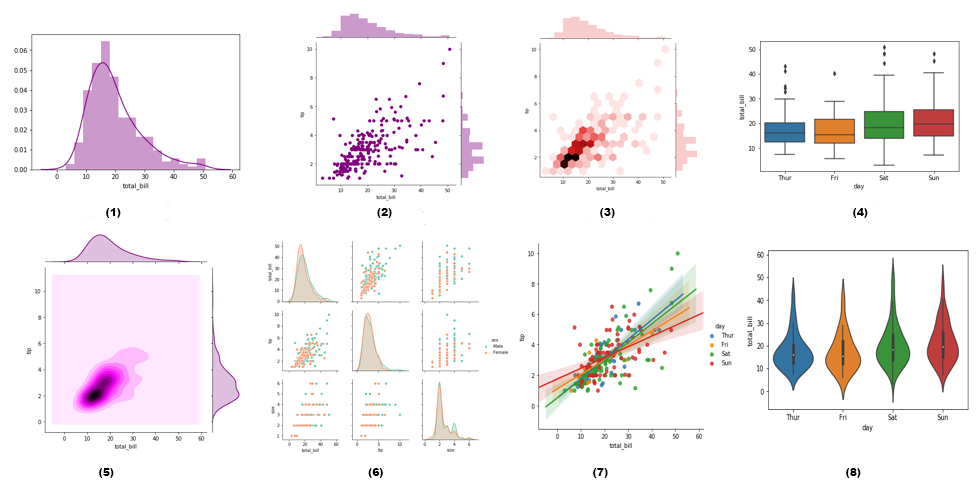
\includegraphics[scale=0.45]{sections/machine-learning/images/seaborn.png}
    \caption{Beispiele für (1) Dist Plots, (2) Hex Plots, (3) Box Plots, (4) KDE Plots, (5) Pair Plots und (6) Violin Plots}
\end{figure}